\chapter{Estado del arte}
\label{sec:estadoArte}
En este apartado lo que pretende es mostrar como se encuentra el panorama en el cual vamos a llevar a cabo este proyecto. Para ello, en primer lugar voy a analizar soluciones similares ya existentes, de forma que analicemos los requisitos de nuestro sistema comparándolo con aquellos que ya existen para obtener nuestra propuesta de valor.

\section{Análisis de mercado}

Como he comentado ya con anterioridad, el acceso a los datos sobre las defunciones es de dominio público, se puede encontrar información al respecto en los sitios que voy a exponer a continuación. Cualquiera puede acceder a ellos y verlos, el principal problema surge cuando queremos hacernos preguntas en base a esos números que vemos. Hasta que nivel se adaptan los sistemas existentes a las necesidades de mis usuarios. Vamos a ver las principales fuentes que existen y lo que nos ofrecen para a continuación, saber que tipo de tratamiento informático necesitamos realizar para satisfacer las necesidades de estos.

\subsection{Instituto Nacional de Estadística}
Uno de los primeros sitios en los que consulté fue la página del \href{https://www.ine.es/index.htm}{Instituto Nacional de Estadística} que es un referente en España en cuanto a la coordinación de servicios estadístico.
En este \href{https://www.ine.es/jaxiT3/Tabla.htm?t=6609}{enlace} se pueden observar las defunciones según causa de muerte filtradas por causa, sexo, edad y periodo. 
Enumero las principales desventajas encontradas desde el punto de vista de mis usuarios:
\begin{itemize}
    \item No permite realizar consultas a los datos.
    \item No soporta ningún protocolo para obtener agnósticamente estos datos y poder usarlo en otros softwares/aplicaciones.
    \item Poca precisión de filtrado por las pocas variables de las que disponemos.
    \item No tenemos visualización gráfica. Te redirige a descargar el programa PC-Axis únicamente disponible para Windows si quieres ver mas detalles sobre los datos almacenados.
\end{itemize}
\FloatBarrier
\begin{figure}[]
	\centering
	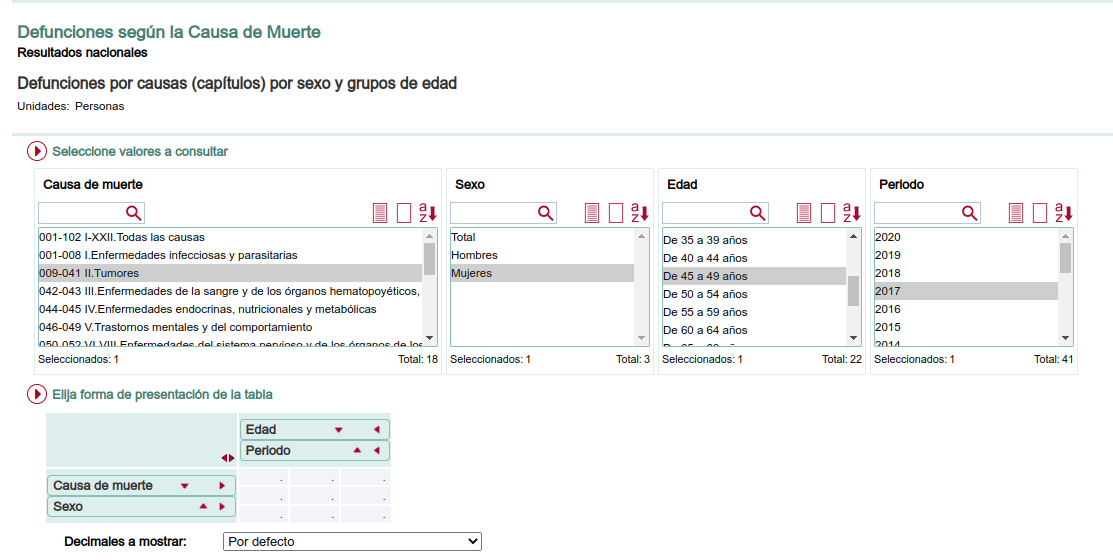
\includegraphics[scale=0.5]{doc/logos/imgs/ine1.png}
	\caption{  Vista principal para obtener datos en el INE }
    \label{fig:worst_f_value}
\end{figure}

\begin{figure}[]
	\centering
	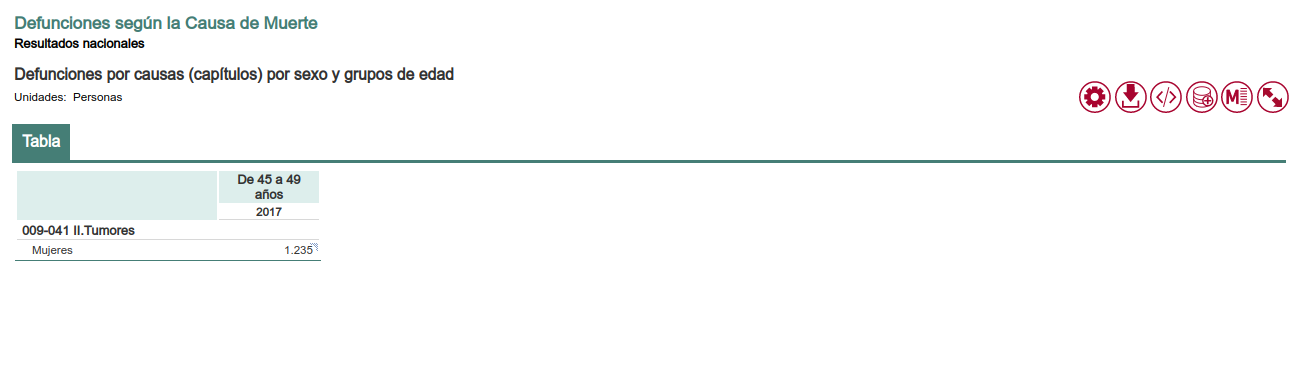
\includegraphics[scale=0.5]{doc/logos/imgs/ine2.png}
	\caption{ Vista resultado cuando se han filtrado los datos a obtener }
    \label{fig:worst_f_value}
\end{figure}
\FloatBarrier

\subsection{Instituto de Salud Carlos III}
En la página del Instituto de Salud Carlos III \footnote{https://www.isciii.es/Paginas/Inicio.aspx} podemos encontrar muchas entradas  hablando sobre \Gls{mortalidad} de la población y \Gls{morbilidad} apoyada de \Gls{momo} \href{https://www.isciii.es/QueHacemos/Servicios/VigilanciaSaludPublicaRENAVE/EnfermedadesTransmisibles/MoMo/Paginas/default.aspx}{Instituto de Salud Carlos III - Vigilancia de la Mortalidad Diaria} que son gráficas de desviaciones de mortalidad diaria respecto a la esperada según las series históricas de mortalidad, estas constituyen un sistema de vigilancia que proporciona información sobre el impacto en mortalidad de la población. Estas son entregables en formato web y PDF.

A pesar de la valiosísima información que estos informes pueden arrojar, sobre todo desde el punto de vista sanitario. Esto no es lo que persigue satisfacer en este trabajo, que se centra en facilitar la obtención de datos crudos. El instituto pone a disposición de los ciudadanos dos servidores.

\subsubsection{Servidor Arïadna}
Nos permite consultar información sobre las causas de defunción atendiendo a cuatro variables: Indicador, Causa, Período y años. Estas variables son las disponibles desde la interfaz web.
Y los indicadores pueden ser:
\begin{enumerate}
  \item Tasa ajustada a la población europea.
  \item Tasa ajustada a la población mundial.
  \item Tasa truncada: tasa ajustada de mortalidad limitada a los 35-64 años de edad.
  \item Índice comparativo de mortalidad: Es el cociente entre la tasa ajustada por edad en cada provincia y la tasa
  ajustada para el conjunto de España.
  \item Tasa cruda: la tasa cruda de mortalidad es la proporción de personas que fallecen con respecto al total
  de la población en un período determinado. Se expresa habitualmente como el número de defunciones al año
  por cada 100.000 personas.
  \item Número de defunciones
\end{enumerate}
\FloatBarrier
\begin{figure}[]
	\centering
	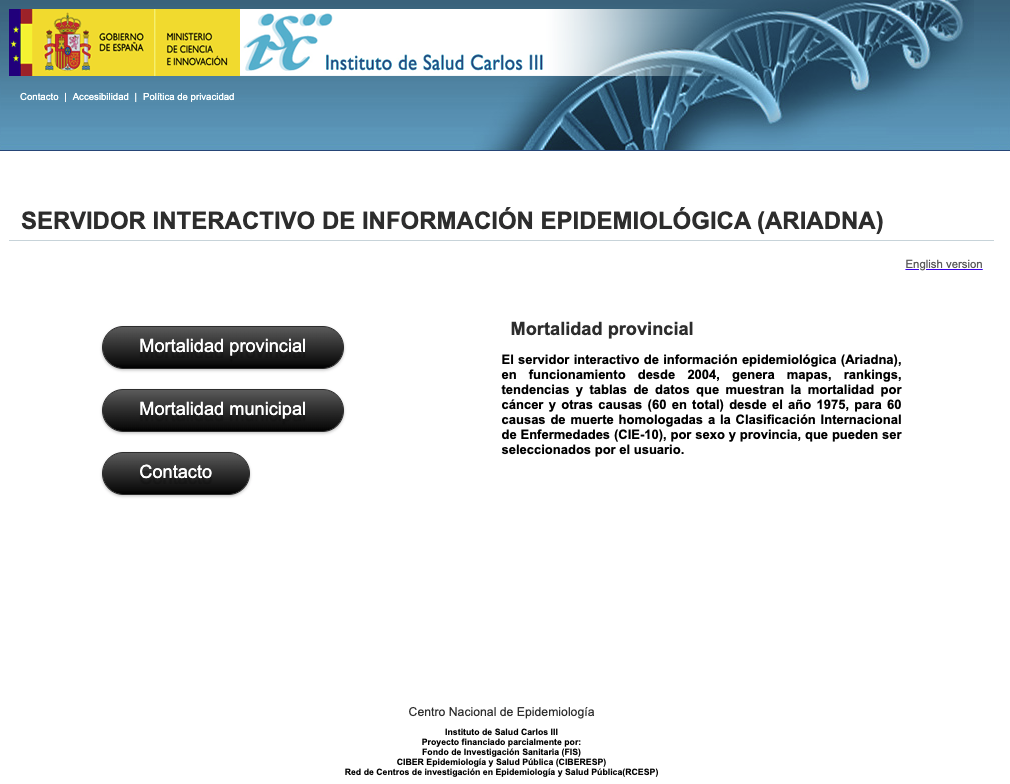
\includegraphics[scale=0.3]{doc/logos/imgs/ariadna1.png}
	\caption{ Vista principal del \href{http://ariadna.cne.isciii.es/}{servidor Arïadna} }
    \label{fig:worst_f_value}
\end{figure}

\begin{figure}[]
	\centering
	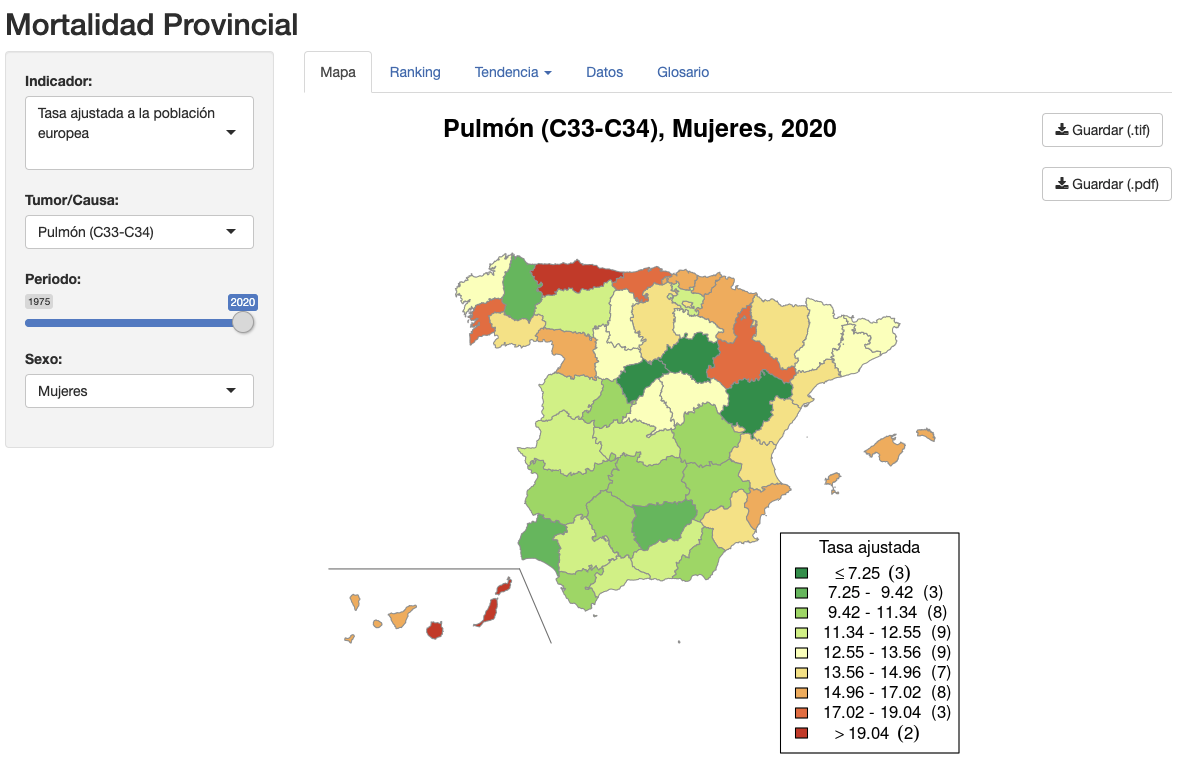
\includegraphics[scale=0.3]{doc/logos/imgs/ariadna2.png}
	\caption{ Vista por mortalidad provincial del servidor Arïadna }
    \label{fig:worst_f_value}
\end{figure}
\FloatBarrier
Los datos son ofrecidos mediante un mapa de España interactivo podemos observar también gráficas de todas las provincias y la media nacional así como una tabla con los datos. Es de obligado comentar la antigüedad manifiesta de la página y la poca agilidad con la que cargan los contenidos.
Esta página permite descargarse los datos únicamente en formato CSV y sólo de 10 tuplas en 10 tuplas sobre las  variables filtradas. Lo que sigue dificultando el acceso completo a cualquier interesado.

\subsubsection{Servidor Raziël}
Es un servidor interactivo \footnote{http://raziel.cne.isciii.es/index.php} que genera mapas y gráficas de España por comunidades autónomas, y tablas de datos que muestran las diferencias en la mortalidad por diversas causas. Ofrece datos desde el año 1980, de acuerdo con los criterios que dé el usuario.
La web nos permite consultar las gráficas citadas anteriormente atendiendo a cuatro variables:
\begin{enumerate}
    \item Indicador.
    \item Causa.
    \item Período, años.
    \item Sexo.
    \item Grupo de edades.
    \item Comunidad Autónoma.
\end{enumerate}

Estas variables son las disponibles desde la interfaz web. Además, la web es prácticamente inaccesible e imposible de obtener los datos en tablas o en algún formato descargable por lo que no me quedó otra opción más que contactar con los servicios informáticos del instituto.


\section{Mi propuesta ante el estado del arte}

Sin perder de vista los \hyperref[sec:obj]{objetivos} y \hyperref[sec:usu]{usuarios diana} a utilizar este trabajo ha sido una tarea útil y fundamental contrastar las "soluciones" existentes para darme cuenta de que los datos no son nada accesibles ni para científicos para que puedan desarrollar estudios ni prácticamente para usuarios observadores ya que la antigüedad de los sistemas, el tiempo de carga y lo nula inversión en accesibilidad hace imposible su uso.

Tras ponerme en contacto con los servicios informáticos del instituto, no tuvieron problema alguno en pasarme todos los ficheros de los que se sirve el servidor, de hecho me llevé una grata sorpresa al ver que almacenaban más variables de las que ellos ofrecían, lo que me ha permitido hacer un trabajo más rico. \hyperref[cap:5]{En el capítulo 5: Análisis de los datos, lo analizaremos más en detalle.}


Para terminar con mi propuesta, he recogido someramente los siguientes puntos en los que ha de guiarse la solución. Las principales deficiencias encontradas y objetivo a subsanar son:
\begin{itemize}
    \item Inexistencia de una interfaz de consulta para que usuarios externos puedan obtener los datos de forma uniforme y utilizando protocolos actuales.
    \item Los datos expuestos en la web no son completos, por razón que desconozco no se muestran todas las variables existentes.
    \item No permite realizar consultas conjuntas a los datos.
    \item La visualización gráfica no se consigue por todas las variables.
\end{itemize}
